\documentclass[a4paper,12pt]{article}
\usepackage[top = 2.5cm, bottom = 2.5cm, left = 2.5cm, right = 2.5cm]{geometry}
% Unfortunately, LaTeX has a hard time interpreting German Umlaute. The following two lines and packages should help. If it doesn't work for you please let me know.
\usepackage[T1]{fontenc}
\usepackage[utf8]{inputenc}
% The following two packages - multirow and booktabs - are needed to create nice looking tables.
\usepackage{multirow} % Multirow is for tables with multiple rows within one cell.
\usepackage{booktabs} % For even nicer tables.
% As we usually want to include some plots (.pdf files) we need a package for that.
\usepackage{graphicx}
\usepackage{tikz}
% The default setting of LaTeX is to indent new paragraphs. This is useful for articles. But not really nice for homework problem sets. The following command sets the indent to 0.
\usepackage[spanish]{babel}
\usepackage{setspace}
\setlength{\parindent}{0in}
% Package to place figures where you want them.
\usepackage{float}
% The fancyhdr package let's us create nice headers.
\usepackage{fancyhdr}
\usepackage{amsmath}
\usepackage{amssymb}
\usepackage{natbib}
\usepackage{apalike}
\usepackage{graphicx}
\usepackage{subcaption}
\usepackage{booktabs}
\usepackage{etoolbox}
\usepackage{amsthm}
\AtBeginEnvironment{align}{\setcounter{equation}{0}}
\newenvironment{solution}
  {\renewcommand\qedsymbol{$\blacksquare$}\begin{proof}[Solución]}
  {\end{proof}}
\pagestyle{fancy}

\fancyhf{}

\lhead{\footnotesize Tarea 3}
\rhead{\footnotesize  Rompich}
\cfoot{\footnotesize \thepage}



\begin{document}
    \thispagestyle{empty} % This command disables the header on the first page.

    \begin{tabular}{p{15.5cm}} % This is a simple tabular environment to align your text nicely
    \begin{tabbing}
    Universidad del Valle de Guatemala 
    \\
    Departamento de Matemática\\ Licenciatura en Matemática Aplicada \\ Fecha de entrega: 5 de marzo de 2021  \\
    Rudik R. Rompich   - Carné: 19857\\
    \end{tabbing}
    Estadística 2 - Eugenio Aristondo \\
    \hline % \hline produces horizontal lines.
    \\
    \end{tabular} % Our tabular environment ends here.
    \vspace*{0.3cm} % Now we want to add some vertical space in between the line and our title.
    \begin{center} % Everything within the center environment is centered.
    {\Large \bf Tarea 3
} % <---- Don't forget to put in the right number
        \vspace{2mm}
    \end{center}
    \vspace{0.4cm}


\section{Capítulo 13}
\subsection{Ejercicio 21}
Considere los resultados experimentales del siguiente diseño de bloques aleatorizado. Realice los cálculos necesarios para establecer la tabla de análisis de varianza. Utilice $\alpha=$ 0.05 para probar cualesquiera diferencias significativas.
\begin{solution}
Considerando: 
\begin{center}
    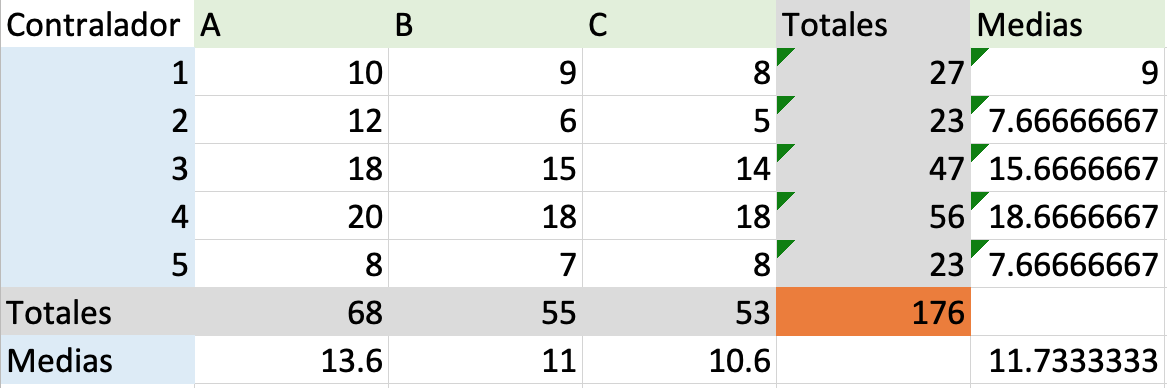
\includegraphics[scale=0.3]{Imagenes/13.png}
\end{center}
Entonces, la construcción de la ANOVA: 

\begin{align}
    \intertext{STC:}
    &= \sum_{i=1}^{b}\sum_{j=1}^{k} (x_{ij}-\overline{\overline{x}})^2 = \sum_{i=1}^{5}\sum_{j=1}^{3} (x_{ij}-\overline{\overline{x}})^2 \\
    &= [(10-11,73)^2+(12-11,73)^2+(18-11,73)^2+(20-11,73)^2+(8-11,73)^2+\\
    & +(9-11,73)^2+(6-11,73)^2+(15-11,73)^2+(18-11,73)^2+(7-11,73)^2+\\
    & +(8-11,73)^2+(5-11,73)^2+(14-11,73)^2+(18-11,73)^2+(8-11,73)^2]\\
    &= 354,93
    \intertext{SCTR:}
    &= b\sum_{j=1}^{k}(x_j-\overline{\overline{x}})^2 = 5\sum_{j=1}^{3}(x_j-\overline{\overline{x}})^2\\
    &= 5[(13,6-11,73)^2+(11-11,73)^2+(10,6-11,73)^2]\\
    &= 26,53
    \intertext{SCBL:}
    &= k\sum_{j=1}^{b}(x_i-\overline{\overline{x}})^2 = 3\sum_{j=1}^{6}(x_i-\overline{\overline{x}})^2\\
    &= 3[(9-11,73)^2+(7,667-11,73)^2+(15,667-11,73)^2+\\
    &+(18,667-11,73)^2+(7,667-11,73)^2]\\
    &= 312,3
    \intertext{SCE:}
    &= STC-SCTR-SCBL\\
    &= 354,93- 26,53-312,3\\
    &= 16,133
\end{align}
Considerando: 
\begin{center}
    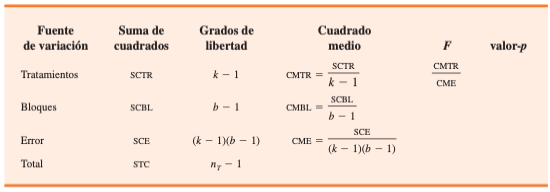
\includegraphics[scale=0.5]{Imagenes/13-1.png}
\end{center}
Entonces, tenemos: 
\begin{center}
    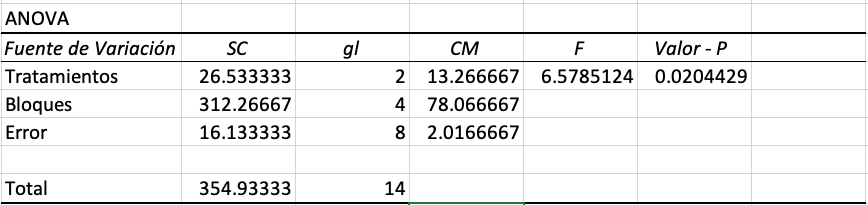
\includegraphics[scale=0.4]{Imagenes/13-2.png}
\end{center}
Buscamos el F crítico: 
\begin{center}
    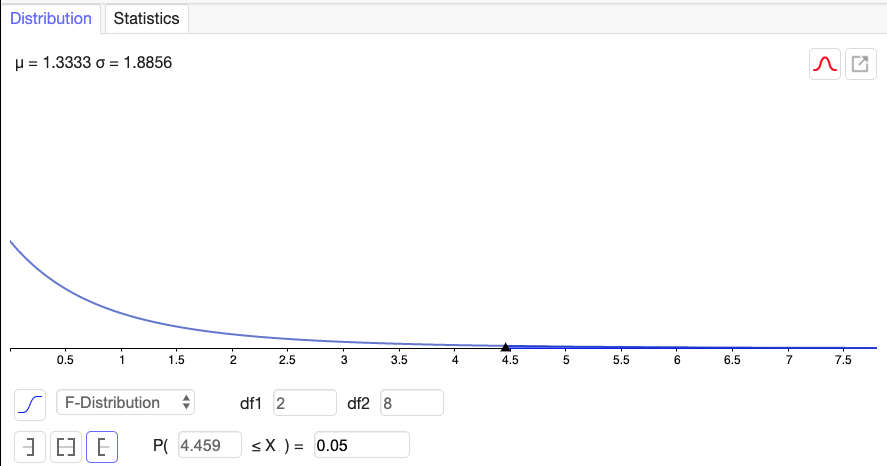
\includegraphics[scale=0.4]{Imagenes/13-3.png}
\end{center}
Es decir, tenemos un $F>F_{\alpha}$. Por lo que se puede concluir que la $H_0$ se rechaza. Las medias son distintas, hay una diferencia significativa entre tratamientos.
\end{solution}
\subsection{Ejercicio 23}
Se realizó un experimento con cuatro tratamientos y ocho bloques. Use $\alpha$ =0.05 y pruebe si existen cualesquiera diferencias significativas. 
\begin{solution}
\begin{align}
    \intertext{SCE:}
    &= STC-SCTR - SCBL\\
    &= 1800-900-400\\
    &= 500
    \intertext{Grados de libertad:}
    k-1 &= 3\\
    b-1 &= 7\\
    (k-1)(b-1) &= 21 \\
    N_t-1 &= 31
    \intertext{Cuadrado medio:}
    CMTR &= \frac{SCTR}{k-1} = \frac{900}{3} =300\\
    CMBL &= \frac{SCBL}{b-1} =\frac{400}{7} = 57,143\\
    CME  &= \frac{SCE}{(k-1)(b-1)} =\frac{500}{21} = 23,81
\intertext{Prueba F:}
 \frac{CMTR}{CME} &= \frac{300}{23,81}=12,6
\end{align}
Entonces, tenemos: 
\begin{center}
    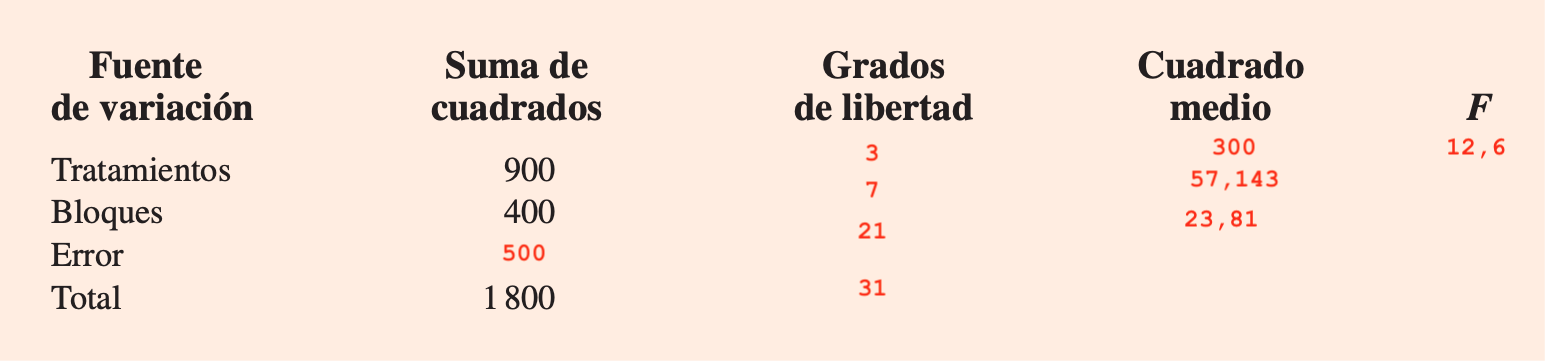
\includegraphics[scale=0.3]{Imagenes/13-4.png}
\end{center}

Entonces, para encontrar el F crítico: 
\begin{center}
    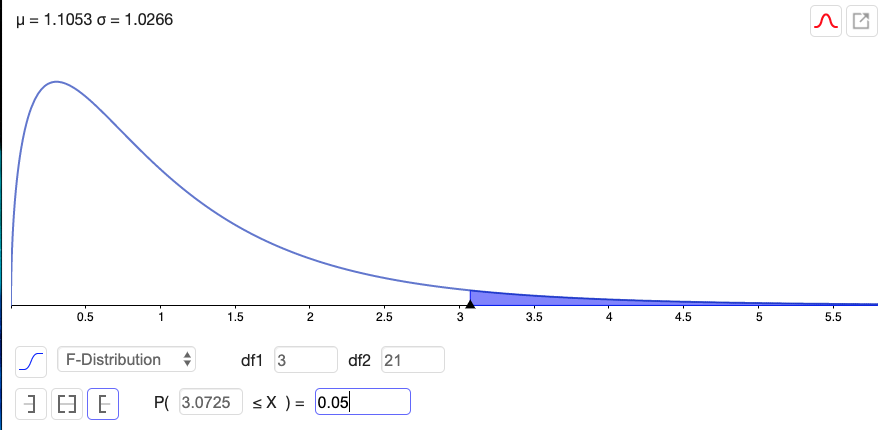
\includegraphics[scale=0.5]{Imagenes/13-5.png}
\end{center}

Por lo tanto, por la prueba F, $F<F_\alpha$. Por lo que las medias son iguales y la $H_0$ se acepta.
\end{solution}
\subsection{Ejercicio 24}
Un vendedor de automóviles realiza una prueba para determinar si el tiempo en minutos que se necesita para afinar un motor pequeño depende de si se utiliza un analizador de motor computarizado o uno electrónico. Debido a que el tiempo de afinación varía entre automóviles compactos, medianos y grandes, en el experimento se utilizaron los tres tipos de vehículos como bloques. Los datos obtenidos se indican a continuación. Use $\alpha =$ 0.05 y pruebe si existen cualesquiera diferencias significativas.

\begin{solution}
Se procede por medio de Excel: 
\begin{center}
    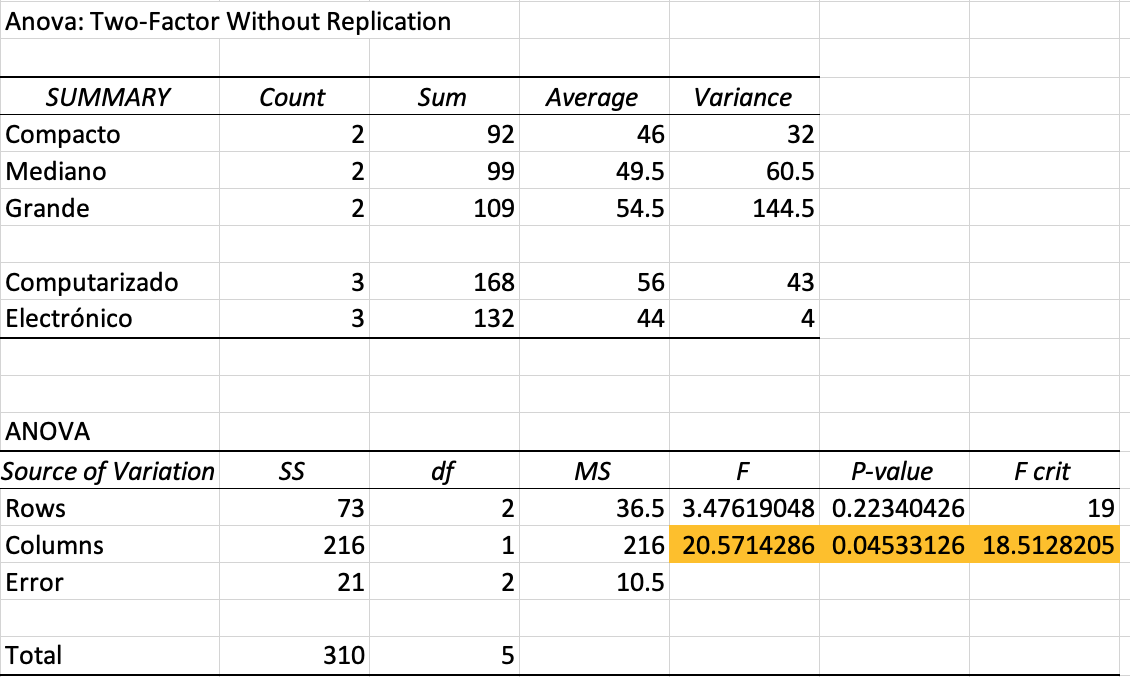
\includegraphics[scale=0.3]{Imagenes/24.png}
\end{center}
\end{solution}

Por lo tanto, por medio de la prueba F; en donde $F>F_\alpha$, es decir, la $H_0$ se rechaza. Existe una diferencia significativa entre tratamientos. Existe una diferencia entre computarizado y electrónico. 

\subsection{Ejercicio 25}
Las vitaminas y otros suplementos para la salud se han encarecido durante los años recientes y, con frecuencia, los precios establecidos por los distintos minoristas varían en gran medida. Los datos a continuación listan los precios de 13 productos (Item) de cuatro minoristas en Rochester, Nueva York (Democrat and Chronicle, 13 de febrero de 2005).
Use $\alpha=$ 0.05 y pruebe si existe alguna diferencia significativa entre los precios medios de los cuatro minoristas.
\begin{solution}
Considerando la solución de Excel: 
\begin{center}
    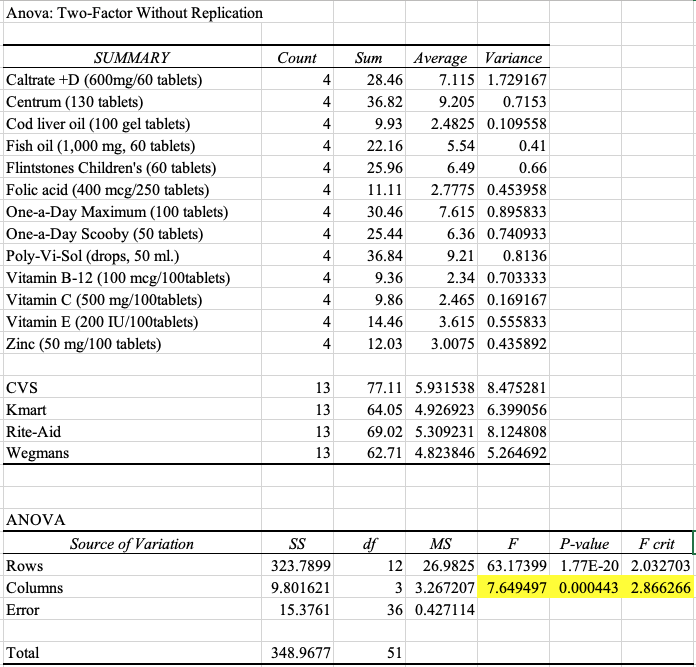
\includegraphics[scale=0.4]{Imagenes/25.png}
\end{center}
Por lo tanto, por medio de la prueba F; en donde $F>F_\alpha$, es decir, la $H_0$ se rechaza. Existe una diferencia significativa entre tratamientos. Es decir, sí existe una diferencia significativa entre los 4 minoritas. 
\end{solution}
\subsection{Ejercicio 26}
 El Examen de aptitud escolar (SAT, por sus siglas en inglés) contiene tres secciones: lectura crítica, matemáticas y redacción. Cada parte se califica en una escala de 800 puntos. La información de las puntuaciones del examen para la versión 2009 del SAT está disponible en el sitio web del College Board. Una muestra de las puntuaciones alcanzadas por seis estudiantes (Student) en el SAT se lista enseguida para lectura crítica (Critical Reading), matemáticas (Mathematics) y redacción (Writing).
 \begin{enumerate}
     \item Utilizando un nivel de significancia de 0.05, ¿los estudiantes se desempeñan de manera distinta en las tres partes del examen?
    \begin{solution}
Considerando la solución de Excel: 
\begin{center}
    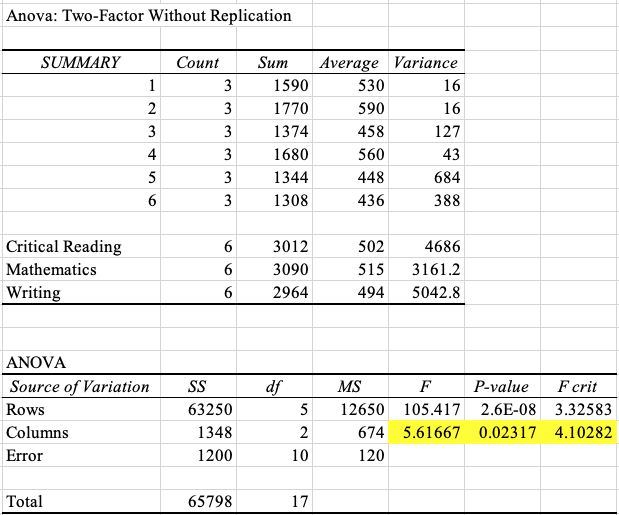
\includegraphics[scale=0.5]{Imagenes/26.png}
\end{center}
Por lo tanto, por medio de la prueba F; en donde $F>F_\alpha$, es decir, la $H_0$ se rechaza. Existe una diferencia significativa entre tratamientos, en otras palabras, el desempeño es distinto en las 3 partes del examen.
    \end{solution}
     \item  ¿Cuál sección parece darles más problemas? Explique.
     \begin{solution}
Según el anterior desarrollo de la ANOVA, la sección de \textit{Writing} tiene la media más pequeña, por lo que se podría inferir que es la sección que da más problemas en el SAT.
\end{solution}
 \end{enumerate}
\subsection{Ejercicio 27}
El Journal of the American Medical Association publicó una investigación acerca de la deman- da cardiaca por palear grandes cantidades de nieve. Diez hombres saludables se sometieron a pruebas de ejercicio empleando una caminadora y una bicicleta adaptada ergonómicamen- te para ejercitar los brazos. Después, estos mismos hombres limpiaron dos tramos de nieve mojada y pesada con una pala ligera para nieve y un lanzanieve eléctrico. Se midió el ritmo cardiaco, la presión sanguínea y el consumo de oxígeno de cada uno de los participantes en la prueba durante la remoción de nieve, y estos valores se compararon con los obtenidos durante las pruebas con la caminadora (Treadmill) y la bicicleta adaptada (Arm-Crank Ergometer). En la tabla siguiente se presentan los valores de ritmo cardiaco expresados en pulsaciones por minuto, de cada uno de los 10 individuos (Subject). Se incluyen los valores de pala para nieve (Snow Shovel) y lanzanieve eléctrico (Snow Thrower).
\begin{solution}
Considerando la solución de Excel: 
\begin{center}
    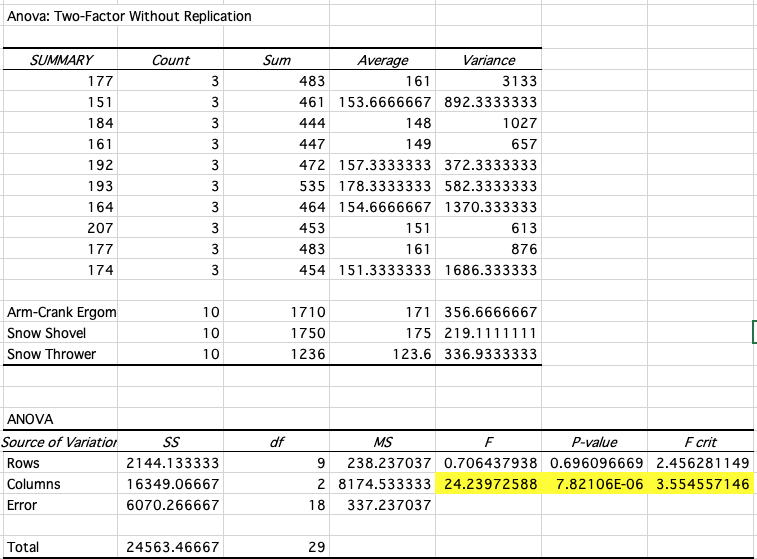
\includegraphics[scale=0.5]{Imagenes/27.png}
\end{center}
\end{solution}

Por lo tanto, por medio de la prueba F; en donde $F>F_\alpha$, es decir, la $H_0$ se rechaza. Existe una diferencia significativa entre tratamientos, en otras palabras sí hay una diferencia significativa entre los cuatro métodos para medir el ritmo cardíaco.
\end{document}